\documentclass{article}
\usepackage[a4paper, total={18cm, 26cm}]{geometry}
\usepackage[utf8]{inputenc}
\usepackage{geometry}
\geometry{hmargin=2cm,vmargin=1.5cm}

%%%%%%%%%%%%%%%%%%%%%%%%%%%%%%%%%%%%%%%%%%%%%%%%%%%%%%%%%%%%%%%%%%%%%%%%%%%
% Support for easy cross-referencing
\usepackage{graphicx}
\usepackage{amsmath}
\usepackage{amssymb}
\usepackage{caption}
\usepackage{booktabs}
\usepackage{nicefrac}
\usepackage{algorithm}
\usepackage[algo2e]{algorithm2e} 
\usepackage{multirow}
\usepackage{mwe}
\usepackage{float}
\usepackage[pagebackref,breaklinks,colorlinks]{hyperref}
\usepackage{ulem}
\usepackage{balance}
\usepackage{comment}
\usepackage{fancyhdr}
\usepackage[capitalize]{cleveref}

%%%%%%%%%%%%%%%%%%%%%%%%%%%%%%%%%%%%%%%%%%%%%%%%%%%%%%%%%%%%%%%%%%%%%%%%%%%
\crefname{section}{Sec.}{Secs.}
\Crefname{section}{Section}{Sections}
\Crefname{table}{Table}{Tables}
\crefname{table}{Tab.}{Tabs.}

%%%%%%%%%%%%%%%%%%%%%%%%%%%%%%%%%%%%%%%%%%%%%%%%%%%%%%%%%%%%%%%%%%%%%%%%%%
\title{Simultaneous Localization And Mapping (SLAM)}
\author{Andreas Birk and Max Pfingsthorn
\thanks{The authors are with the Dept. of Electrical Engineering and Computer Science, Jacobs University Bremen, 28751
Bremen, Germany. {\tt\small
a.birk@jacobs-university.de}}}
\date{November 2022}
\nocite{*}


\begin{document}

\maketitle
%%%%%%%%% ABSTRACT %%%%%%%%%%%%%%%%%%%%%%%%%%%%%%%%%%%%%%%%
\begin{abstract}
This article gives an overview introduction to Simultaneous Localization And Mapping (SLAM), i.e., probabilistic methods to generate a 2D or 3D map of unknown areas under imperfect localization. The article provides a survey of the theoretical basis of SLAM as well as the core background information about the underlying techniques for implementing actual SLAM systems
\end{abstract}

%%%%%%%%%%%%%%%%%%%%%%%%%%%%%%%%Introduction %%%%%%%%%%%%%%%%%%%%%%%%%%%%%%%%%%%%%%%%%%%%%%

\section{\label{sec:intro}Introduction}
Simultaneous Localization And Mapping (SLAM) deals with the chicken and egg problem of building a map, which requires localization, while using this map for localization.  
The term SLAM is used for the problem itself as well as for the algorithmic solutions trying to solve it.  
The term originated in the robotics community but there are strong links to other research areas where the problem is also investigated, respectively where SLAM algorithms that originated in robotics research are used for other mobile systems than robots.  
Examples include Geosciences,especially Geodesy and Geomatics, or Automotive Engineering, especially with respect to building road data bases for car navigation systems and the increasing trend towards autonomous driving.  
In general, the task is to localize a mobile system, which may have any kind of propulsion system.  
Application examples hence cover all forms of ground, aerial, and marine robots.  
But applications of SLAM also include human operated vehicles like cars or the option to place a sensor suite manually at different locations in the environment, e.g., in surveying applications.
SLAM  has  also  been  performed  in  multiple  applications  using  pedestrians  as  mobile  platform  or  while  moving sensors by hand around objects.  In the following, we will refer to the to be localized platform simply as the “robot”for the sake of convenience.

The  robot  has  at  any  moment \textit{t} in time  a  6  degree  of  freedom  (6-DoF)  position  and  orientation  in  3D space  -  or  short  pose $\mathbf{x}_{t}$ -  consisting  of  its  Cartesian  coordinates  and  its  Roll-Pitch-Yaw  (RPY)  angles,  i.e., $\mathbf{x}_{t}=(x_{1},x_{2},x_{3},\theta_{R},\theta_{P},\theta_{Y})^{T}$.   
We  assume  without  loss  of  generality  that $\mathbf{x}_{0}=0$.   
Historically  and  from  the viewpoint of a significant amount of application examples,  a substantial part of SLAM research concentrates on only 2D space, i.e., a 3-DoF robot pose with $\mathbf{x}_{t}=(x_{0},x_{1},\theta)^{T}$.

The robot has one or multiple sensors with which it observes its environment.  
The sensor readings at time t are denoted with ${z}_{t}$.  The sensor readings are processed into a map ${m}_{t}$.  
There are in principle two different ways in which environment observations can be incorporated into SLAM $\left(\cref{fig:Triangle}\right)$.  
First, the environment sensor(s) can recognize and localize natural landmarks, i.e., environment features that can be identified at fixed locations.  
This can for example be a visually distinct spot in the environment that is detected and localized via a stereo camera on the robot.  
Two subsequent observations of this landmark at times $t$ and $t + 1$ allow to estimate the relative motion $\delta\mathbf{x}_{t}$ of the robot, i.e., the relative change in poses that is denoted as follows: $\mathbf{x}_{t}=\mathbf{x}_{t}\oplus\delta\mathbf{x}_{t}$.

An essential element of SLAM is to consider the uncertainty of each motion estimate, respectively of each pose estimate derived from it.  
We can therefore associate a probability distribution $P(\mathbf{x}_t)$ for each time step t.  
The robot’s motions over time or short trajectory from the start $t= 0$ to a moment $t=k$ leads to a sequence of poses or short a path that is denoted with $\mathbf{x}_{0:k}$.  The related environment observations,  control inputs,  and maps are accordingly denoted with $\mathbf{z}_{0:k}$,$\mathbf{u}_{0:k}$, and $\mathbf{m}_{0:k}$.  
Each sequential motion estimate increases the uncertainty in the robot’s  localization. \cref{fig:Rond} shows  an  example  where  we  assume  a  Gaussian  distribution  for  the  pose  estimates.
The Covariance in $\mathbf{x}_{0}$ and $\mathbf{x}_{1}$, i.e., along the Cartesian x- and y-axis, can then be illustrated using ellipses - the orientation $\theta$ is omitted for the sake of simplicity.  
Each motion estimate introduces additional uncertainty and the overall error grows in an unbounded fashion.

%%%%%%%%%%%%%%%%%%%%%%%%%%%%%%%% SLAM %%%%%%%%%%%%%%%%%%%%%%%%%%%%%%%%%%%%%%%%%%%%%%

\section{\label{sec:SLAM Fronted}SLAM Frontend}

\subsection{Egomotion Estimation with Internal Sensors and Models}
For mobile robots, the process of estimating their motion from internal sensors - also known as interoceptive sensors in contrast to exteroceptive or external environment sensors - is known as odometry [1, 2].  Given motor control inputut $\mathbf{x}_{t}$, respectively actual motor speeds measured by rotational encoders, the robots motion can be determined


\begin{figure}[H]
    \centering
    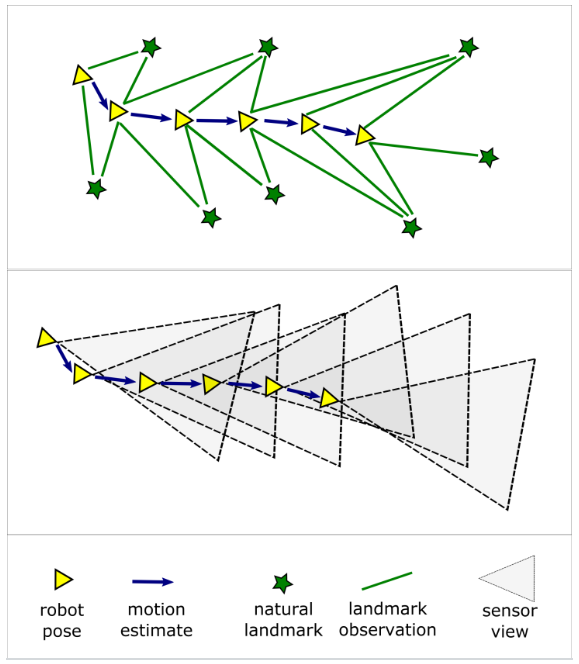
\includegraphics{image/Triangle.png}
    \caption{Environment sensors can be incorporated in two substantially different ways to perform SLAM. 
    First, there is  the  option  to  recognize  and  localize  landmarks,  i.e.,  fixed  unique  locations  in  the  environment,  to  estimate  the motion of the robot (top).  Second,  constraints can be generated by registration,  i.e.,  the spatial alignment of two overlapping sensor readings (bottom).}
    \label{fig:Triangle}
\end{figure}


\begin{figure}[H]
    \centering
    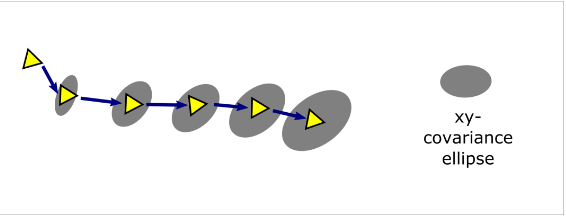
\includegraphics{image/Rond.PNG}
    \caption{SLAM uncertainty}
    \label{fig:Rond}
\end{figure}

\begin{figure}[H]
    \centering
    \begin{tabular}{ccc}
         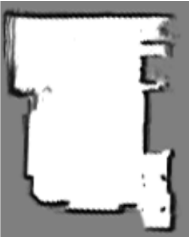
\includegraphics{image/a.PNG}   
         &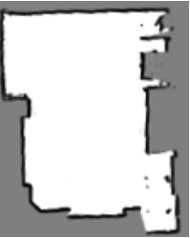
\includegraphics{image/b.PNG} 
         &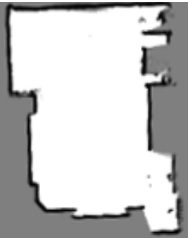
\includegraphics{image/c.PNG} 
         \\ (a) & (b) & (c) \\
         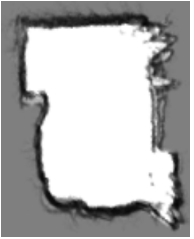
\includegraphics{image/d.PNG} 
         &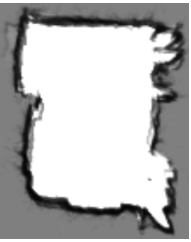
\includegraphics{image/e.PNG} 
         &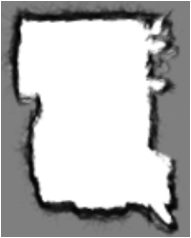
\includegraphics{image/f.PNG} 
         \\ (d) & (e) & (f)
    \end{tabular}
    %\captionsetup[width=18cm]
    \caption{Comparisons of map constructed from ZED scan(down) and LIDAR scan(top).  (a)LIDAR scan; (b)LIDARscan + ZED odom; (c) LIDAR scan + ZED odom + IMU; (d)ZED scan; (e)ZED scan + ZED odom; (f)ZED scan +ZED odom + IMU.}
    \label{fig:fig3}
\end{figure}


by forward kinematics.  
An important example is the differential drive (also known as a kinematic cart), i.e., a robot with two wheels that can be driven at different speeds.  
The control inputs, respectively measured speed, for the left and the right motor are sampled at fixed time intervals $\delta t$.  
Given the mechanical set-up of the gearbox and the wheel diameter, the motor-speeds can be used to determine the distances $s_{l}$, respectively $s_{r}$ the left, respectively right wheel traveled in the time interval.  
Given the constant distance $b$ between the two wheels, the change in pose $\delta x_{t}= (\delta x_{0},\delta x_{1},\delta \theta)^{T}$ can be computed as follows [3]:

%%%%%%%%%%%%%%%%%%%%%%%%%%%%%%%%%%%ù Equation1 %%%%%%%%%%%%%%%%%%%%%%%%%%%%%%%%%%%%%%%
\begin{equation}
\mathbf{x_{t+1}}=\mathbf{x_{t}}+\mathbf{\delta x_{t}}=\mathbf{x_{t}}+\left(\begin{array}{c}
     s \cos{\left( \theta_{t}+\delta\theta/2\right)}
     \\
     s \sin{\left(\theta_{t}+\delta\theta/2\right)}
     \\
     \delta\theta
     \\
\end{array}
  \right)
  \label{eq:equation1}
\end{equation}
with
\begin{equation}
    \mathbf{s}=\frac{\mathbf{s_{r}}+\mathbf{s_{r}}}{2}\;and\;\delta\theta =\frac{\mathbf{s_{r}}-\mathbf{s_{l}}}{b} \nonumber
\end{equation}
%%%%%%%%%%%%%%%%%%%%%%%%%%%%%%%%%%%%%%%%%%%%%%%%%%%%%%%%%%%%%%%%%%%%%%%%%%%%%%%%%%%%%

Given two parameters $k_{r}$ and $k_{l}$ to cover probabilistic aspects of the motor drive and of the wheel-floor inter-action, the following covariance matrix $\Sigma_{s}$ can be assumed for the motion increment:

%%%%%%%%%%%%%%%%%%%%%%%%%%%%%%%%%%%ù Equation2 %%%%%%%%%%%%%%%%%%%%%%%%%%%%%%%%%%%%%%%
\begin{equation}
    \Sigma_{s}=\left(\begin{array}{cc}
    k_{r}s_{r} & 0
    \\
     0 & k_{l}s_{l}
     \\
    \end{array}
    \right)
\end{equation}
%%%%%%%%%%%%%%%%%%%%%%%%%%%%%%%%%%%%%%%%%%%%%%%%%%%%%%%%%%%%%%%%%%%%%%%%%%%%%%%%%%%%%


%%%%%%%%%%%%%%%%%%%%%%%%%%%%%%%%%%% Experimental results %%%%%%%%%%%%%%%%%%%%%%%%%%%%
\section{\label{sec:Experimental results}Experimental results}
As is known, the quality of the map depends heavily on the initial pose of AGV. The odometry was recognized as one of the methods that could provide high precision pose estimation in a short period of time.  Similarly, the accurate orientation of AGV could also be provided by IMU. Therefore, the maps built by algorithms combining the odometry and IMU are superior to those built by single sensor-based algorithms.An intuitive observation of above maps did not help us determine which was the best choice.  Next, the lengths of maps generated above were also compared with the ground truth, and the metric, calculating the proportion of occupied cells in map as the sum of occupied cells divided by number of free cells (see, \cref{eq:eq3}), as described in the paper [3] were used to compare the quality of above maps.  Generally, the proportion of occupied cells correspond to the quality of the map:  the higher this proportion – the lower quality of the map.  And it should be noted that the metric calculating the proportion of occupied cells should be used only as a part of a complex analysis.


%%%%%%%%%%%%%%%%%%%%%%%%%%%%%%%%%%% Tableau %%%%%%%%%%%%%%%%%%%%%%%%%%%%
\begin{table}[H]
    \centering
    \begin{tabular}{clcccc}
        \hline
        &Combinations & Measure(m) & Truth(m)  & Error(m) & Proportion(\%) 
        \\
        \hline
        \multirow{2}{*}{LIDAR} & LIDAR scan & 5.722 & 5.901 & 0.179 & 13.6
        \\
        \multirow{2}{*}{combinations}& LIDAR scan + ZED odom & 5.808 & 5.901 & 0.093 & 10.0
        \\
         & LIDAR scan + ZED odom + IMU & 5.827 & 5.901 & 0.074 & 10.7
         \\
        \multirow{2}{*}{ZED} & ZED scan & 5.405 & 5.901 & 0.496 & 19.9
        \\
        \multirow{2}{*}{combinations}& ZED scan + ZED odom & 5.655 & 5.901 & 0.246 & 19.6
        \\ 
         & ZED scan + ZED odom + IMU & 5.667 & 5.901 & 0.234 & 20.4
         \\   
        \hline
    \end{tabular}
    \caption{Cumulative errors and the proportion of occupied cells for each combination.}
    \label{tab:tableauMulti}
\end{table}

%%%%%%%%%%%%%%%%%%%%%%%%%%%%%%%%%%%%%% Equation 3 %%%%%%%%%%%%%%%%%%%%%%%%%%%%%%%%%%%%%%%%%%%%%%%%%%%
\begin{equation}
prop\left(occupied\right)=\frac{Number\left(occupied\_cells\right)}{Number\left(free\_cells\right)}
    \label{eq:eq3}
\end{equation}
%%%%%%%%%%%%%%%%%%%%%%%%%%%%%%%%%%%%%%%%%%%%%%%%%%%%%%%%%%%%%%%%%%%%%%%%%%%%%%%%%%%%%%%%%%%%%%%%%%%%%

The  experimental  results  were  classified  by  different  sensor  combinations  applied,  which  were  presented  in \cref{tab:tableauMulti}.  
The algorithm combing the LIDAR, ZED odometry, and IMU showed the best mapping performance in all combinations with a minimum cumulative mapping error of 0.074.  
The mapping performance of the algorithm using LIDAR combinations with a mean cumulative error around 0.11 was better than the algorithm using ZED combinations  mean  cumulative  error  with  around  0.32.   
Next,  from  the  last  column  in  \cref{tab:tableauMulti},  it  could  be  seen that the mean proportion of occupied cells of ZED combinations was almost twice that of LIDAR combinations,implying that the maps generated by algorithms based on LIDAR combinations had a little blurry effect.



\end{document}

